\documentclass[border=8pt]{standalone}
\usepackage{amsmath,amssymb,bm}
\usepackage{xcolor}
\usepackage{tikz}
\definecolor{P}{HTML}{4B1D8F}
\definecolor{ink}{HTML}{1B1B2F}
\definecolor{X}{HTML}{C2386B}
\colorlet{rule}{P!45!white}
\begin{document}
\Large
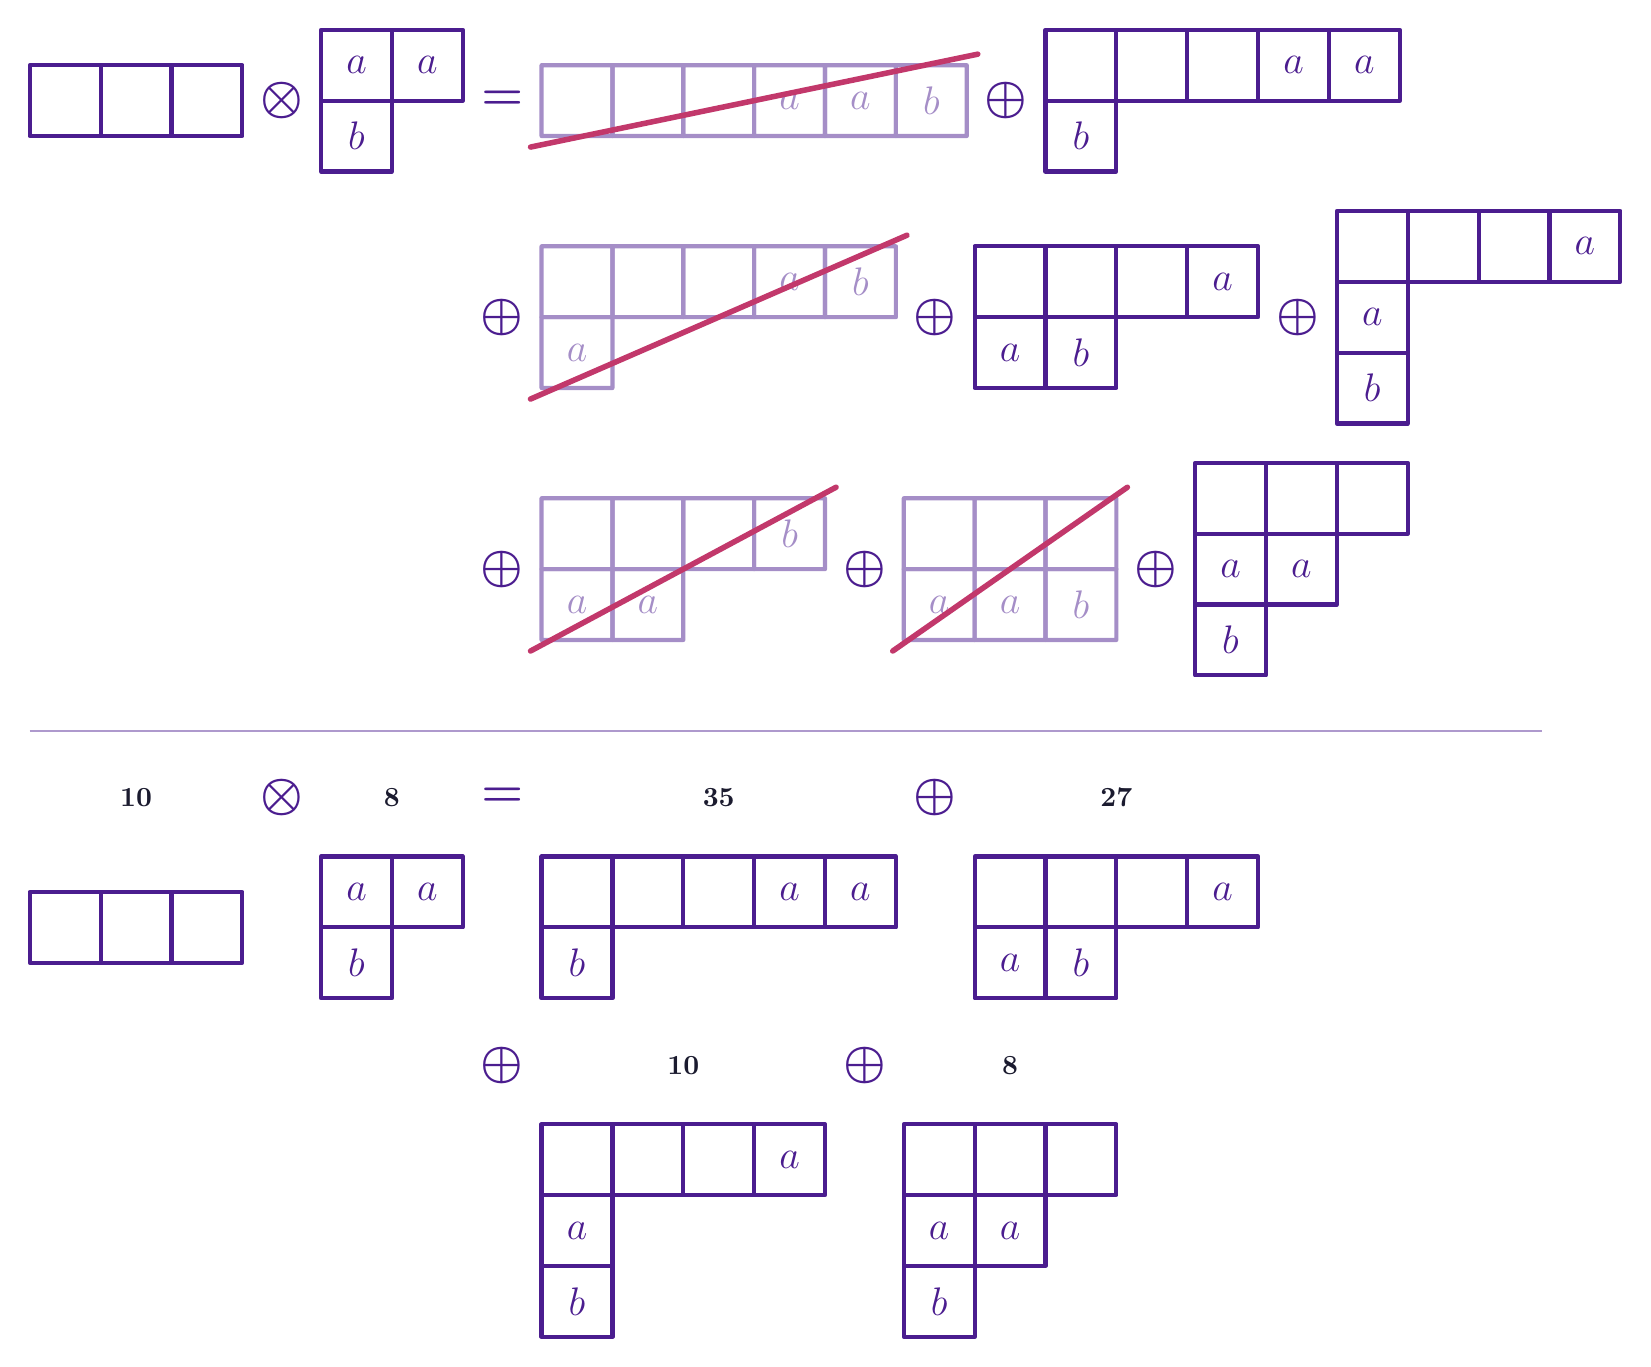
\begin{tikzpicture}[every node/.style={text=ink}]
\draw[P,line width=1.5pt,line join=round] (0.000,0.450) rectangle (0.900,-0.450);
\draw[P,line width=1.5pt,line join=round] (0.900,0.450) rectangle (1.800,-0.450);
\draw[P,line width=1.5pt,line join=round] (1.800,0.450) rectangle (2.700,-0.450);
\node[text=P] at (3.200,0.000) {\LARGE$\bm{\otimes}$};
\draw[P,line width=1.5pt,line join=round] (3.700,0.900) rectangle (4.600,0.000);
\node[text=P] at (4.150,0.450) {\Large$a$};
\draw[P,line width=1.5pt,line join=round] (4.600,0.900) rectangle (5.500,0.000);
\node[text=P] at (5.050,0.450) {\Large$a$};
\draw[P,line width=1.5pt,line join=round] (3.700,0.000) rectangle (4.600,-0.900);
\node[text=P] at (4.150,-0.450) {\Large$b$};
\node[text=P] at (6.000,0.000) {\LARGE$\bm{=}$};
\begin{scope}[transparency group,opacity=.5]
\draw[P,line width=1.5pt,line join=round] (6.500,0.450) rectangle (7.400,-0.450);
\draw[P,line width=1.5pt,line join=round] (7.400,0.450) rectangle (8.300,-0.450);
\draw[P,line width=1.5pt,line join=round] (8.300,0.450) rectangle (9.200,-0.450);
\draw[P,line width=1.5pt,line join=round] (10.100,0.450) rectangle (11.000,-0.450);
\node[text=P] at (10.550,0.000) {\Large$a$};
\draw[P,line width=1.5pt,line join=round] (9.200,0.450) rectangle (10.100,-0.450);
\node[text=P] at (9.650,0.000) {\Large$a$};
\draw[P,line width=1.5pt,line join=round] (11.000,0.450) rectangle (11.900,-0.450);
\node[text=P] at (11.450,0.000) {\Large$b$};
\end{scope}
\draw[X,line width=2pt,line cap=round] (6.360,-0.590) -- (12.040,0.590);
\node[text=P] at (12.400,0.000) {\LARGE$\bm{\oplus}$};
\draw[P,line width=1.5pt,line join=round] (12.900,0.900) rectangle (13.800,0.000);
\draw[P,line width=1.5pt,line join=round] (13.800,0.900) rectangle (14.700,0.000);
\draw[P,line width=1.5pt,line join=round] (14.700,0.900) rectangle (15.600,0.000);
\draw[P,line width=1.5pt,line join=round] (16.500,0.900) rectangle (17.400,0.000);
\node[text=P] at (16.950,0.450) {\Large$a$};
\draw[P,line width=1.5pt,line join=round] (15.600,0.900) rectangle (16.500,0.000);
\node[text=P] at (16.050,0.450) {\Large$a$};
\draw[P,line width=1.5pt,line join=round] (12.900,0.000) rectangle (13.800,-0.900);
\node[text=P] at (13.350,-0.450) {\Large$b$};
\node[text=P] at (6.000,-2.750) {\LARGE$\bm{\oplus}$};
\begin{scope}[transparency group,opacity=.5]
\draw[P,line width=1.5pt,line join=round] (6.500,-1.850) rectangle (7.400,-2.750);
\draw[P,line width=1.5pt,line join=round] (7.400,-1.850) rectangle (8.300,-2.750);
\draw[P,line width=1.5pt,line join=round] (8.300,-1.850) rectangle (9.200,-2.750);
\draw[P,line width=1.5pt,line join=round] (6.500,-2.750) rectangle (7.400,-3.650);
\node[text=P] at (6.950,-3.200) {\Large$a$};
\draw[P,line width=1.5pt,line join=round] (9.200,-1.850) rectangle (10.100,-2.750);
\node[text=P] at (9.650,-2.300) {\Large$a$};
\draw[P,line width=1.5pt,line join=round] (10.100,-1.850) rectangle (11.000,-2.750);
\node[text=P] at (10.550,-2.300) {\Large$b$};
\end{scope}
\draw[X,line width=2pt,line cap=round] (6.360,-3.790) -- (11.140,-1.710);
\node[text=P] at (11.500,-2.750) {\LARGE$\bm{\oplus}$};
\draw[P,line width=1.5pt,line join=round] (12.000,-1.850) rectangle (12.900,-2.750);
\draw[P,line width=1.5pt,line join=round] (12.900,-1.850) rectangle (13.800,-2.750);
\draw[P,line width=1.5pt,line join=round] (13.800,-1.850) rectangle (14.700,-2.750);
\draw[P,line width=1.5pt,line join=round] (12.000,-2.750) rectangle (12.900,-3.650);
\node[text=P] at (12.450,-3.200) {\Large$a$};
\draw[P,line width=1.5pt,line join=round] (14.700,-1.850) rectangle (15.600,-2.750);
\node[text=P] at (15.150,-2.300) {\Large$a$};
\draw[P,line width=1.5pt,line join=round] (12.900,-2.750) rectangle (13.800,-3.650);
\node[text=P] at (13.350,-3.200) {\Large$b$};
\node[text=P] at (16.100,-2.750) {\LARGE$\bm{\oplus}$};
\draw[P,line width=1.5pt,line join=round] (16.600,-1.400) rectangle (17.500,-2.300);
\draw[P,line width=1.5pt,line join=round] (17.500,-1.400) rectangle (18.400,-2.300);
\draw[P,line width=1.5pt,line join=round] (18.400,-1.400) rectangle (19.300,-2.300);
\draw[P,line width=1.5pt,line join=round] (16.600,-2.300) rectangle (17.500,-3.200);
\node[text=P] at (17.050,-2.750) {\Large$a$};
\draw[P,line width=1.5pt,line join=round] (19.300,-1.400) rectangle (20.200,-2.300);
\node[text=P] at (19.750,-1.850) {\Large$a$};
\draw[P,line width=1.5pt,line join=round] (16.600,-3.200) rectangle (17.500,-4.100);
\node[text=P] at (17.050,-3.650) {\Large$b$};
\node[text=P] at (6.000,-5.950) {\LARGE$\bm{\oplus}$};
\begin{scope}[transparency group,opacity=.5]
\draw[P,line width=1.5pt,line join=round] (6.500,-5.050) rectangle (7.400,-5.950);
\draw[P,line width=1.5pt,line join=round] (7.400,-5.050) rectangle (8.300,-5.950);
\draw[P,line width=1.5pt,line join=round] (8.300,-5.050) rectangle (9.200,-5.950);
\draw[P,line width=1.5pt,line join=round] (6.500,-5.950) rectangle (7.400,-6.850);
\node[text=P] at (6.950,-6.400) {\Large$a$};
\draw[P,line width=1.5pt,line join=round] (7.400,-5.950) rectangle (8.300,-6.850);
\node[text=P] at (7.850,-6.400) {\Large$a$};
\draw[P,line width=1.5pt,line join=round] (9.200,-5.050) rectangle (10.100,-5.950);
\node[text=P] at (9.650,-5.500) {\Large$b$};
\end{scope}
\draw[X,line width=2pt,line cap=round] (6.360,-6.990) -- (10.240,-4.910);
\node[text=P] at (10.600,-5.950) {\LARGE$\bm{\oplus}$};
\begin{scope}[transparency group,opacity=.5]
\draw[P,line width=1.5pt,line join=round] (11.100,-5.050) rectangle (12.000,-5.950);
\draw[P,line width=1.5pt,line join=round] (12.000,-5.050) rectangle (12.900,-5.950);
\draw[P,line width=1.5pt,line join=round] (12.900,-5.050) rectangle (13.800,-5.950);
\draw[P,line width=1.5pt,line join=round] (11.100,-5.950) rectangle (12.000,-6.850);
\node[text=P] at (11.550,-6.400) {\Large$a$};
\draw[P,line width=1.5pt,line join=round] (12.000,-5.950) rectangle (12.900,-6.850);
\node[text=P] at (12.450,-6.400) {\Large$a$};
\draw[P,line width=1.5pt,line join=round] (12.900,-5.950) rectangle (13.800,-6.850);
\node[text=P] at (13.350,-6.400) {\Large$b$};
\end{scope}
\draw[X,line width=2pt,line cap=round] (10.960,-6.990) -- (13.940,-4.910);
\node[text=P] at (14.300,-5.950) {\LARGE$\bm{\oplus}$};
\draw[P,line width=1.5pt,line join=round] (14.800,-4.600) rectangle (15.700,-5.500);
\draw[P,line width=1.5pt,line join=round] (15.700,-4.600) rectangle (16.600,-5.500);
\draw[P,line width=1.5pt,line join=round] (16.600,-4.600) rectangle (17.500,-5.500);
\draw[P,line width=1.5pt,line join=round] (14.800,-5.500) rectangle (15.700,-6.400);
\node[text=P] at (15.250,-5.950) {\Large$a$};
\draw[P,line width=1.5pt,line join=round] (15.700,-5.500) rectangle (16.600,-6.400);
\node[text=P] at (16.150,-5.950) {\Large$a$};
\draw[P,line width=1.5pt,line join=round] (14.800,-6.400) rectangle (15.700,-7.300);
\node[text=P] at (15.250,-6.850) {\Large$b$};
\draw[rule,line width=.7pt] (0,-8.000) -- (19.200,-8.000);
\draw[P,line width=1.5pt,line join=round] (0.000,-10.050) rectangle (0.900,-10.950);
\draw[P,line width=1.5pt,line join=round] (0.900,-10.050) rectangle (1.800,-10.950);
\draw[P,line width=1.5pt,line join=round] (1.800,-10.050) rectangle (2.700,-10.950);
\node at (1.350,-8.850) {$\mathbf{10}$};\node[text=P] at (3.200,-8.850) {\LARGE$\bm{\otimes}$};
\draw[P,line width=1.5pt,line join=round] (3.700,-9.600) rectangle (4.600,-10.500);
\node[text=P] at (4.150,-10.050) {\Large$a$};
\draw[P,line width=1.5pt,line join=round] (4.600,-9.600) rectangle (5.500,-10.500);
\node[text=P] at (5.050,-10.050) {\Large$a$};
\draw[P,line width=1.5pt,line join=round] (3.700,-10.500) rectangle (4.600,-11.400);
\node[text=P] at (4.150,-10.950) {\Large$b$};
\node at (4.600,-8.850) {$\mathbf{8}$};\node[text=P] at (6.000,-8.850) {\LARGE$\bm{=}$};
\node at (8.750,-8.850) {$\mathbf{35}$};
\draw[P,line width=1.5pt,line join=round] (6.500,-9.600) rectangle (7.400,-10.500);
\draw[P,line width=1.5pt,line join=round] (7.400,-9.600) rectangle (8.300,-10.500);
\draw[P,line width=1.5pt,line join=round] (8.300,-9.600) rectangle (9.200,-10.500);
\draw[P,line width=1.5pt,line join=round] (10.100,-9.600) rectangle (11.000,-10.500);
\node[text=P] at (10.550,-10.050) {\Large$a$};
\draw[P,line width=1.5pt,line join=round] (9.200,-9.600) rectangle (10.100,-10.500);
\node[text=P] at (9.650,-10.050) {\Large$a$};
\draw[P,line width=1.5pt,line join=round] (6.500,-10.500) rectangle (7.400,-11.400);
\node[text=P] at (6.950,-10.950) {\Large$b$};
\node[text=P] at (11.500,-8.850) {\LARGE$\bm{\oplus}$};
\node at (13.800,-8.850) {$\mathbf{27}$};
\draw[P,line width=1.5pt,line join=round] (12.000,-9.600) rectangle (12.900,-10.500);
\draw[P,line width=1.5pt,line join=round] (12.900,-9.600) rectangle (13.800,-10.500);
\draw[P,line width=1.5pt,line join=round] (13.800,-9.600) rectangle (14.700,-10.500);
\draw[P,line width=1.5pt,line join=round] (12.000,-10.500) rectangle (12.900,-11.400);
\node[text=P] at (12.450,-10.950) {\Large$a$};
\draw[P,line width=1.5pt,line join=round] (14.700,-9.600) rectangle (15.600,-10.500);
\node[text=P] at (15.150,-10.050) {\Large$a$};
\draw[P,line width=1.5pt,line join=round] (12.900,-10.500) rectangle (13.800,-11.400);
\node[text=P] at (13.350,-10.950) {\Large$b$};
\node[text=P] at (6.000,-12.250) {\LARGE$\bm{\oplus}$};
\node at (8.300,-12.250) {$\mathbf{10}$};
\draw[P,line width=1.5pt,line join=round] (6.500,-13.000) rectangle (7.400,-13.900);
\draw[P,line width=1.5pt,line join=round] (7.400,-13.000) rectangle (8.300,-13.900);
\draw[P,line width=1.5pt,line join=round] (8.300,-13.000) rectangle (9.200,-13.900);
\draw[P,line width=1.5pt,line join=round] (6.500,-13.900) rectangle (7.400,-14.800);
\node[text=P] at (6.950,-14.350) {\Large$a$};
\draw[P,line width=1.5pt,line join=round] (9.200,-13.000) rectangle (10.100,-13.900);
\node[text=P] at (9.650,-13.450) {\Large$a$};
\draw[P,line width=1.5pt,line join=round] (6.500,-14.800) rectangle (7.400,-15.700);
\node[text=P] at (6.950,-15.250) {\Large$b$};
\node[text=P] at (10.600,-12.250) {\LARGE$\bm{\oplus}$};
\node at (12.450,-12.250) {$\mathbf{8}$};
\draw[P,line width=1.5pt,line join=round] (11.100,-13.000) rectangle (12.000,-13.900);
\draw[P,line width=1.5pt,line join=round] (12.000,-13.000) rectangle (12.900,-13.900);
\draw[P,line width=1.5pt,line join=round] (12.900,-13.000) rectangle (13.800,-13.900);
\draw[P,line width=1.5pt,line join=round] (11.100,-13.900) rectangle (12.000,-14.800);
\node[text=P] at (11.550,-14.350) {\Large$a$};
\draw[P,line width=1.5pt,line join=round] (12.000,-13.900) rectangle (12.900,-14.800);
\node[text=P] at (12.450,-14.350) {\Large$a$};
\draw[P,line width=1.5pt,line join=round] (11.100,-14.800) rectangle (12.000,-15.700);
\node[text=P] at (11.550,-15.250) {\Large$b$};
\end{tikzpicture}
\end{document}
